\begin{figure}
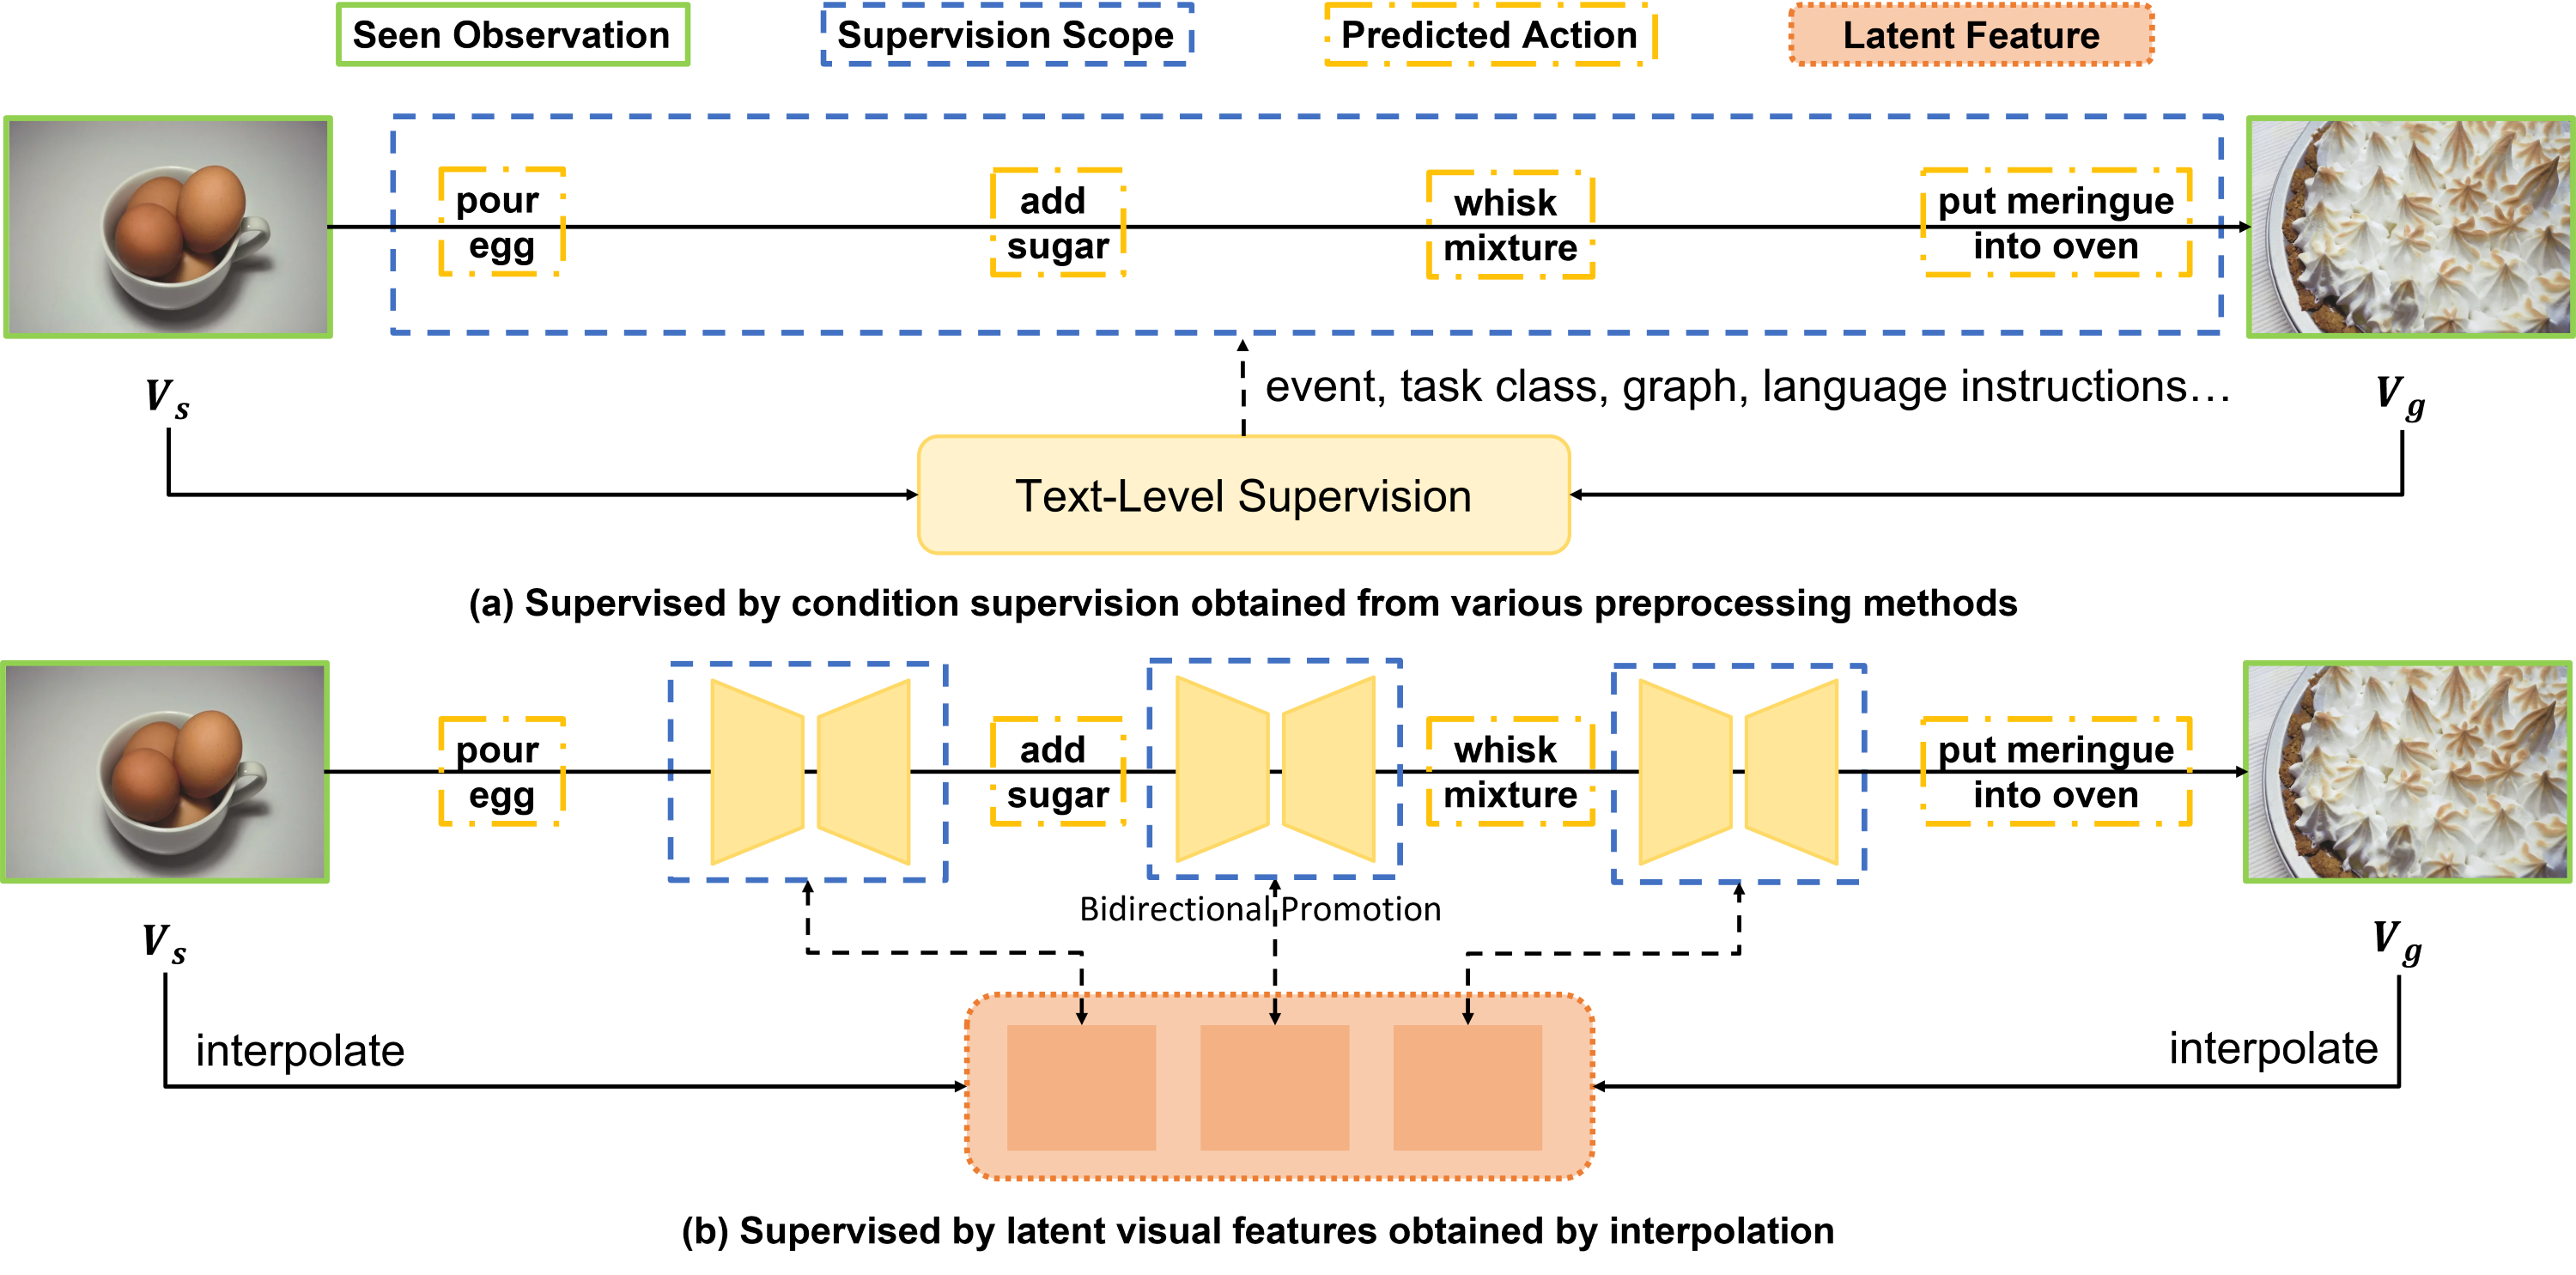
\includegraphics[width=0.98\textwidth, height=0.49\textheight]{figures/fig-task.png}
\vspace{-0.5em}
\caption{(a) The procedure planning is to predict a sequence of action steps given the language instructions. (b) For the full supervision setting, intermediate visual observations are annotated with timestamps in the videos. (c) For the state supervisions, LLMs-generated descriptions are annotated and taken for state representation learning. (d) We leverage the latent frames from interpolation and class labels from classifier as supervisions.}
\label{fig:task}
\vspace{-4mm}
\end{figure}



% \begin{figure}[h]
% \begin{center}
% \framebox[4.0in]{$\;$}
% \fbox{\rule[-.5cm]{0cm}{4cm} \rule[-.5cm]{4cm}{0cm}}
% \end{center}
% \caption{Sample figure caption.}
% \end{figure}

% Figure 1. Procedure planning example. Given a start observationOstart and a goal state ogoal, the model is required to generatea sequence of actions that can transform ostart to ogoal. Previousapproaches rely on heavy intermediate supervision during training,while our model only needs the task class labels (bottom row).